% mainfile: ../ltexpprt.tex


\subsection{Experimental Setup}
 In this paper, we concentrated on 15 Latin
American countries viz. Argentina, Bolivia, Costa Rica, Colombia, Chile,
Ecuador,  El Salvador, Guatemala, French Guiana, Honduras, Mexico, Nicaragua,
Paraguay, Panama and Peru. We collected weekly Influenza estimates (ILI counts)
from the official Pan American Health Organization (PAHO)
website~\cite{PAHO:2013}, every day from January 2013 to August 2013. The
estimates downloaded every day contain data from January 2010 to the last
available week for the said day, for each country under consideration. The
downloaded data is next pre-processed to fill ILI counts for any missing weeks
using linear interpolation. This dataset is stored in a database we refer to as
``Temporal Data Repository'' (TDR) .  The TDR is also timestamped so that for
any given day between the said period, we can readily retrieve the ILI case
counts that were download on the same day since historic data may be updated by
PAHO long after the week observed.  For the purpose of experimental validation
we used the data for the period Jan 2010 to December 2012 as the static
training set. We considered Wednesdays of the weeks as our time points.  For
each Wednesday from Jan 2013 to July 2013, we used the latest available PAHO
data in TDR for that day and predicted 3 weeks from the last available week for
which the PAHO data was available. These predictions are next evaluated against
the final ILI case count as downloaded on September 1, 2013 and we report the
performance of our algorithms in Section~\ref{sec:results}. 

\subsection{Evaluation criteria}
 We evaluated the prediction accuracy of the
different algorithms using a modified version of ``Percentage Relative Error''.
Using the notation as explained earlier and listed in Table~\ref{tb:notations}
we defined the accuracy metric as given in equation~\ref{eq:def:accuracy}.

\begin{equation} 
    \label{eq:def:accuracy} 
    \mathcal{A} = \frac{4}{N_p}\sum \limits_{t=t_s}^{t_e}\frac{|P_t -\hat{P}_t| }{max(P_t, \hat{P}_t, 10)}
\end{equation} 
where, $t_s$ and $t_e$ indicates the starting and the ending
time point for which predictions were generated.  $N_p$ indicates the number of
time points over the same time period (i.e. $N_p = t_e - t_s + 1$). 

The accuracy criterion was designed according the following criteria:
\begin{itemize} 
    \item 
    The accuracy estimates should reflect the percentage
    deviation in prediction rather than absolute deviation. 
     \prithwish{should we justify this?} 
\item The accuracy estimates must be non-negative.  \item If we
don't consider the max operator in the denominator, even ``good'' predictions
such as 1 for an actual count of 0 will be assigned an accuracy score of 0. As
such we chose a threshold (here 10) for which very small deviations are not
over-penalized. The threshold was chosen by manually inspecting the span of ILI
case counts (which were found to lie between 0 and 2000) and subsequent
feedback from subject experts about the ``interesting'' range of predictions.
\end{itemize} 
It is to be noted that the accuracy metric so defined is
non-convex and was found to be multi-modal. 


\subsection{Surrogate Data sources}
For the algorithm we described in Section~\ref{sec:methods},
we used a number of different data sources as
surrogates. We considered a wide range for such surrogates comprising both
physical indicators such as weather characteristics, and also non-physical
indicators such as social network activities and user search queries.  For a
number of the non-physical indicators such as Twitter activities, the most
important part is to properly identify the keywords associated with flu so that
we can get a proper estimate of the flu-related surrogate information. This key
step is described in section~\ref{sec:keyword}, and is followed by an
explanation of the surrogates sources in section. 

\subsubsection{\label{sec:keyword} Keywords Extraction} % mainfile: ../ltexpprt.tex

The keywords relating to ILI were
organized from a seed set of words and expanded using a combination of 
time-series correlation analysis and pseudo-query expansion.
The seed set of keywords (e.g., {\em gripe}) was constructed in Spanish, 
Portugese, and English using feedback from our 
in-house subject mattter expers.

\paragraph{Pseudo-query expansion.}
Using the seed set, we crawled
the top 20 web sites (according to Google Search) associated with each
word in this set. We also crawled some expert sites such as the official CDC
website and equivalent websites of the countries under consideration, detailing the
causes, symptoms and treatment for influenza.
Additionally we crawled a few hand-picked websites such as
\url{http://www.flufacts.com} and \url{http://health.yahoo.net/channel/flu\_treatments}.
We filtered the words from these sites using standard language
processing filtering techniques such as stopword removal and Porter
stemming. The filtered set of keywords were then ranked according to 
the absolute frequency of occurrence. The top 500 words for Spanish and
English were then selected. For example, words such as {\em enfermedad}
and {\em pandemia} were obtained from this step.

\paragraph{Time-series correlation analysis.}
Next we used Google Correlate (now a part of Google Trends) to identify keywords
most correlated with
the ILI case count time-series for each country.
Once again these words were found to be a mix of 
 both English and Spanish. As an added step in this process, we also
 compared time-shifted ILI counts: left-shifted  to capture the words searched leading up to 
 the actual flu infection and right-shifted to capture the words
commonly searched during the tail of the infection. 
This entire exercise provided us some interesting terms like {\em ginger} which has been used as
a natural herbal remedy in the eastern world. We also found popular flu medications
such as {\em Acemuk} and  {\em Oseltamivir}, which are also sold under the trade name of
{\em Tamiflu} as highly correlated search queries, especially particularly for
Argentina.

\paragraph{Final filtering.}
The set of terms obtained from query expansion and correlation analysis were then 
pruned by hand to obtain a vocabulary of 151 words. We then performed a final
correlation check and retained a final set of 114 words.



We next describe the different data sources.

\subsubsection{Google Flu Trends ($\mathcal{F}$) :}
Google Flu Trends~\cite{GFT:2013} (GFT) is a tool based
on~\cite{ginsberg2008detecting} and provided by Google.org which gives weekly
and up-to-date ILI case count estimates using search query volumes. As
mentioned in~\cite{ginsberg2008detecting}, GFT is based on a regression model
from search query estimates to actual ILI case counts.  Of the countries under
consideration, GFT provides weekly estimates for 6 of them viz.  Argentina,
Bolivia, Chile, Mexico, Peru and Paraguay. As mentioned in
Table.~\ref{tb:notations}, we denote the weekly estimate of GFT data for the
country under consideration by $\mathcal{F} = \langle \mathcal{F}_1,
\mathcal{F}_2, \dots, \mathcal{F}_{T1} \rangle$. This estimate is typically at
a different scale than the ILI case counts provided by PAHO and therefore needs
to be scaled accordingly.  We collected this data weekly on Monday from Jan
2013 to Aug 2013. The data downloaded on a particular day contains the entire
time-series from 2004 to the corresponding week.  
 

\subsubsection{Google Search Trends ($\mathcal{S}$) :} Google Search Trends~\cite{GST:2013} is
another tool provided by Google. Using this tool we can download an estimate of
search query volume as a percentage over its own temporal history. This
download can be further filtered geographically over a country.  We download
the search query volumes for the 114 keywords as described in
Section~\ref{sec:keyword} every week and convert the percentage measures to
absolute values using a static dataset we downloaded on Oct 2012 when Google
Search Trends used to provide absolute relative values of query volumes. The
time series constructed using this dataset, for the country under consideration
is denoted by
$\mathcal{S} = \langle \mathcal{S}_1, \mathcal{S}_2, \dots, \mathcal{S}_{T1} \rangle$.

\subsubsection{Twitter ($\mathcal{T}$) :} 
We also collected Twitter data from Datasift~\cite{Twitter:2013},
one of the certified data resellers for
Twitter data. Using a paid data collection API, we can specify queries in
Datasift and get the corresponding filtered data.  We started with a mix of
queries targeted at collecting data from only the countries under
consideration. Using our in-house Geo coders we next processed the collected
Tweets to specific countries and then using syntactic analyzers from Basis
Enrichment~\cite{Basis:2013} we parsed the Tweet contents into ``lemma'' - root
forms of words, and also detected the Language and the part of speech for the
word under consideration.  Importantly, the Basis Enrichment step allows
differentiation between different languages (for example the Spanish word
``gripe'', meaning flu, is part of our flu keyword as opposed to the undesired
and unrelated English word ``gripe''). Also using the lemmatized versions we
can match between different parts-of-speech variations of the same word. Using
the lemma sized equivalents of our keyword dictionary we next parsed the
enriched Tweets for possible matches with flu related keywords and constructed
a time series of flu keyword weekly occurrence count. For the country under
consideration, we denote this time series by 
$\mathcal{T} = \langle \mathcal{T}_1, \mathcal{T}_2, \dots, \mathcal{T}_{T1} \rangle$.

We started collecting flu filtered Tweeter Data from November 2012 and everyday
we download the corresponding Twitter time-series for each country. As shown in
Figure~\ref{fig:ili_data_pipeline}, every week we collect 10GB of raw Twitter
Data which are next enriched to 20GB of structured data. From this dataset, we
parse flu-related Tweets resulting in around 7GB of data. This data is finally
abstracted into a multivariate time series over lemmatized versions of the 114
flu related keywords and added to the TDR. 

\subsubsection{HealthMap ($\mathcal{H}$) :} 
Similar to Twitter data, we also collect flu-related
news stories using HealthMap~\cite{HM:2013}, an online global disease alert
system capturing outbreak data from over 50,000 electronic sources [including
  expert-curated accounts, such as ProMED-Mail~\cite{chase1996promed}, news media
and official reports from local, national and global public health
organizations.] Using this service we receive flu-related news as a daily feed
which is similarly processed using Basis Enrichment and further filtered to get
a multivariate time series over  lemmatized version of the keywords. For a
particular country, we denote this time series by: 
$\mathcal{H} = \langle \mathcal{H}_1, \mathcal{H}_2, \dots, \mathcal{H}_{T1} \rangle$.

While Twitter Data is more suitable to look for general public response, the
HealthMap data provides more detailed information but may capture the trends
more slowly than the Twitter Data. Thus each of these sources offers utility in
capturing different surrogate signals: Twitter Data offers leading but noisy
indicators whereas HealthMap Data provides a slightly delayed but more reliable
indicator.

\subsubsection{OpenTable ($\mathcal{O}$) :}
We also use data on trends of restaurant table reservations, as initially 
found in~\cite{elaine2013opentable} to be a potential early indicator for
outbreak surveillance, as another surrogate for ILI detection.
This novel data stream is based on the
postulate that higher than average number of restaurants with table
availabilities in a region can serve as an indicator of an event of interest
such as increase in flu cases. Table availability was monitored using OpenTable
~\cite{Opentable:2013}; an online restaurant reservation site with 28,000 restaurants at the time
of this writing. Daily searches were performed starting from September 2012 for
a table for two persons at lunch and dinner; between 12:30-3pm, and between
6-10:30pm. Data was collected for Mexico by city (Cancun, Mexico City, Puebla,
Monterrey, and Guadalajara) and for the entire country. The daily proportion
(proportion used due to changes in the number of restaurants in the system) of
restaurants with available tables was aggregated as a weekly time-series and
is denoted by 
$\mathcal{O} = \langle \mathcal{O}_1, \mathcal{O}_2, \dots, \mathcal{O}_{T1} \rangle$.


%--Since we monitored ten regions at twenty search times, this resulted in 200
%distinct time-series curves.
\begin{figure} 
  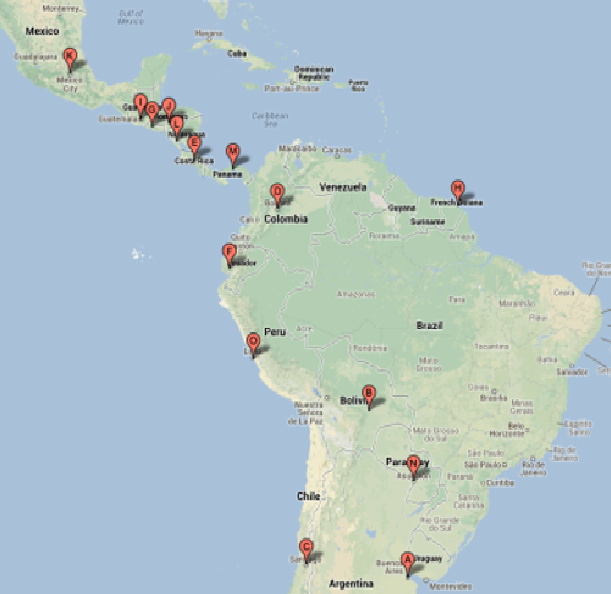
\includegraphics[width=3.33in]{fig/humidity_centers.pdf}
  \caption{\label{fig:surveillance} PAHO surveillance centers for the 15 Latin
  American countries.}
\end{figure}

\subsubsection{Weather Data ($\mathcal{W}$) :}
All of the previously described data sources can
be termed as `non-physical' indicators. These data sources can work as indirect
indicators about the state of the population with respect to flu by exposing
different population characteristics. At the same time, meteorological data can
be considered a more direct and `physical' driver of influenza transmission
~\cite{flu_humidity_physical}. It has been shown
in~\cite{Shaman_orig_humidity_link, Shaman_humidity_USA, ref9}
that absolute humidity can be directly used to predict the onset of influenza
epidemics. Here, we collected several other meteorological factors such as
temperature and rainfall in addition to humidity from the Global Data
Assimilation System (GDAS) which is a series of weather models run by National
Weather Service's National Centers for Environmental Prediction that provides
detailed meteorological data in near real-time across the globe.  We accessed
the data via an archive hosted by NASA (http://ladsweb.nascom.nasa.gov/)
~\cite{HD:2013}, and provided in GRIB format. By specifying the resolution and
the geographical boundaries we can collect the data for the countries under
consideration to a resolution of 1 degrees lat/long interval. However, looking
at all the lat/long for a country can often lead to noisy data. As such we
filtered the downloaded data and parsed the meteorological data only around the
PAHO surveillance centers as shown in Figure~\ref{fig:surveillance}. We also
aggregate this data using weekly averages and for a particular country we
represent the time resultant time series by: 
$\mathcal{W} = \langle \mathcal{W}_1, \mathcal{W}_2, \dots, \mathcal{W}_{T1} \rangle$.

We collected this data weekly from Jan 2013 to August 2013. 


\subsubsection{Temporal Data Repository}
All of the described data sources were
added to a temporal database, ``Temporal Data Repository'' (TDR). Some of the
data sources such as the Weather Data, Twitter Data, HealthMap Data and
OpenTable data once downloaded doesn't change. Also at the time of download
these datasets are updated till the corresponding day.  Thus to extract the
data available at a certain time point for these data sets we can simply
consider the corresponding truncated time series from the latest data. However,
Statistics like Google Search Trends and the PAHO ILI case counts exhibit
variability in past data. Thus the actual time series for these datasets are
stored in TDR with the corresponding timestamps. Thus given any time point,
using TDR we can quickly reference the data available at that point of time and
run our algorithm to simulate a prospective analysis scenario.  The entire data
collection process is depicted pictorially in
Figure~\ref{fig:ili_data_pipeline}.



